
%(BEGIN_QUESTION)
% Copyright 2015, Tony R. Kuphaldt, released under the Creative Commons Attribution License (v 1.0)
% This means you may do almost anything with this work of mine, so long as you give me proper credit

Read and outline the ``Connector and Tip Styles'' subsection of the ``Thermocouples'' section of the ``Continuous Temperature Measurement'' chapter in your {\it Lessons In Industrial Instrumentation} textbook.  Note the page numbers where important illustrations, photographs, equations, tables, and other relevant details are found.  Prepare to thoughtfully discuss with your instructor and classmates the concepts and examples explored in this reading.


\underbar{file i03988}
%(END_QUESTION)





%(BEGIN_ANSWER)


%(END_ANSWER)





%(BEGIN_NOTES)

Thermocouples are typically packaged with stainless-steel sheaths to protect the junction from damage.  The tips of these sheathed thermocouples may be either grounded (connected to the sheath) or ungrounded.  Grounded tips exhibit faster response times than ungrounded tips, but are susceptible to electrical ground loops.  Exposed tips are the fastest of all, but are fragile.

\vskip 10pt

Quick-disconnect thermocouple connectors are ``polarized'' with different-sized plug contacts, to discourage wrong polarity.

\vskip 10pt

Most thermocouple wire assemblies use solid wire rather than stranded, and therefore must never be crimped inside of a compression lug (terminal).  The proper termination method for solid wire at a screw is to wrap the wire around the screw and let it be directly compressed by the screw head.



\vskip 20pt \vbox{\hrule \hbox{\strut \vrule{} {\bf Suggestions for Socratic discussion} \vrule} \hrule}

\begin{itemize}
\item{} Explain how thermocouple plugs are built to ensure they are plugged in correctly, and not backwards.
\item{} Suppose a thermocouple were wired into a circuit ``backwards''.  What would be the effect?  Sketch an iron-copper junction circuit to prove to yourself what would happen if you did.
\item{} Identify correct and incorrect applications for a ``crimp'' style electrical connecting lug.
\item{} Explain in thermodynamic terms why grounded-tip thermocouples have faster response times than ungrounded-tip thermocouples.
\item{} Identify both correct and incorrect methods to connect {\it solid} thermocouple wires together in a circuit.
\end{itemize}







\vfil \eject

In order to answer the backwards-connected thermocouple question, here are a pair of diagrams showing correct versus incorrect connections for an iron-copper thermocouple:

$$\includegraphics[width=15.5cm]{i03988x01.eps}$$

Connecting a thermocouple backwards produces {\it two} forward-facing (measurement) junctions at the plug and {\it two} reverse-facing (reference) junctions (one at the tip, the other at the meter).

%INDEX% Reading assignment: Lessons In Industrial Instrumentation, Continuous Temperature Measurement (thermocouples)

%(END_NOTES)


